\documentclass[tikz,border=8pt]{standalone}
% Shared look for every TikZ diagram. Load with % Shared look for every TikZ diagram. Load with % Shared look for every TikZ diagram. Load with \input{../../tools/tikz-style.tex}
\usepackage[T1]{fontenc}
\usepackage{lmodern}
\renewcommand{\sfdefault}{lmr}  % diagrams use the same serif as the text
\usetikzlibrary{arrows.meta, positioning, shapes.geometric, calc, fit, backgrounds}
\definecolor{cblue}{HTML}{4C78A8}
\definecolor{corange}{HTML}{F58518}
\definecolor{cgreen}{HTML}{54A24B}
\definecolor{cred}{HTML}{E45756}
\definecolor{cpurple}{HTML}{B279A2}
\definecolor{cgrey}{HTML}{6B6B6B}
\tikzset{
  every picture/.style={font=\sffamily, line width=1.2pt},
  box/.style={draw=#1, fill=#1!12, rounded corners=4pt, align=center, inner sep=7pt, minimum height=1.1cm},
  box/.default=cgrey,
  arrow/.style={-{Stealth[length=3mm]}, draw=cgrey, line width=1.4pt},
  title/.style={font=\sffamily\bfseries\Large},
  note/.style={font=\sffamily\small, text=cgrey, align=center},
}
\AtBeginDocument{\hyphenpenalty=10000 \exhyphenpenalty=10000}

\usepackage[T1]{fontenc}
\usepackage{lmodern}
\renewcommand{\sfdefault}{lmr}  % diagrams use the same serif as the text
\usetikzlibrary{arrows.meta, positioning, shapes.geometric, calc, fit, backgrounds}
\definecolor{cblue}{HTML}{4C78A8}
\definecolor{corange}{HTML}{F58518}
\definecolor{cgreen}{HTML}{54A24B}
\definecolor{cred}{HTML}{E45756}
\definecolor{cpurple}{HTML}{B279A2}
\definecolor{cgrey}{HTML}{6B6B6B}
\tikzset{
  every picture/.style={font=\sffamily, line width=1.2pt},
  box/.style={draw=#1, fill=#1!12, rounded corners=4pt, align=center, inner sep=7pt, minimum height=1.1cm},
  box/.default=cgrey,
  arrow/.style={-{Stealth[length=3mm]}, draw=cgrey, line width=1.4pt},
  title/.style={font=\sffamily\bfseries\Large},
  note/.style={font=\sffamily\small, text=cgrey, align=center},
}
\AtBeginDocument{\hyphenpenalty=10000 \exhyphenpenalty=10000}

\usepackage[T1]{fontenc}
\usepackage{lmodern}
\renewcommand{\sfdefault}{lmr}  % diagrams use the same serif as the text
\usetikzlibrary{arrows.meta, positioning, shapes.geometric, calc, fit, backgrounds}
\definecolor{cblue}{HTML}{4C78A8}
\definecolor{corange}{HTML}{F58518}
\definecolor{cgreen}{HTML}{54A24B}
\definecolor{cred}{HTML}{E45756}
\definecolor{cpurple}{HTML}{B279A2}
\definecolor{cgrey}{HTML}{6B6B6B}
\tikzset{
  every picture/.style={font=\sffamily, line width=1.2pt},
  box/.style={draw=#1, fill=#1!12, rounded corners=4pt, align=center, inner sep=7pt, minimum height=1.1cm},
  box/.default=cgrey,
  arrow/.style={-{Stealth[length=3mm]}, draw=cgrey, line width=1.4pt},
  title/.style={font=\sffamily\bfseries\Large},
  note/.style={font=\sffamily\small, text=cgrey, align=center},
}
\AtBeginDocument{\hyphenpenalty=10000 \exhyphenpenalty=10000}

\usetikzlibrary{matrix}
\begin{document}
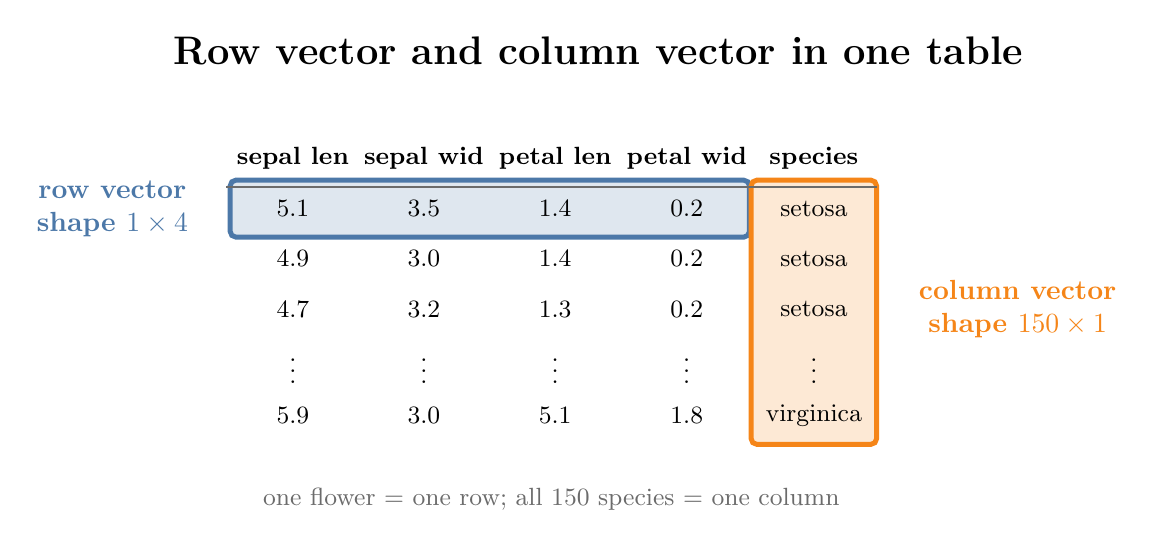
\begin{tikzpicture}
  \node[title] at (0.6,3.0) {Row vector and column vector in one table};
  \matrix (m) [matrix of nodes, nodes={minimum width=1.55cm, minimum height=0.68cm, font=\small, anchor=center},
               column sep=-\pgflinewidth, row sep=-\pgflinewidth] at (0,0) {
    |[font=\small\bfseries]| sepal len & |[font=\small\bfseries]| sepal wid & |[font=\small\bfseries]| petal len & |[font=\small\bfseries]| petal wid & |[font=\small\bfseries]| species \\
    5.1 & 3.5 & 1.4 & 0.2 & setosa \\
    4.9 & 3.0 & 1.4 & 0.2 & setosa \\
    4.7 & 3.2 & 1.3 & 0.2 & setosa \\
    $\vdots$ & $\vdots$ & $\vdots$ & $\vdots$ & $\vdots$ \\
    5.9 & 3.0 & 5.1 & 1.8 & virginica \\
  };
  \begin{scope}[on background layer]
    \fill[cblue!18] (m-2-1.north west) rectangle (m-2-4.south east);
    \fill[corange!18] (m-2-5.north west) rectangle (m-6-5.south east);
  \end{scope}
  \draw[cblue, line width=1.8pt, rounded corners=2pt] (m-2-1.north west) rectangle (m-2-4.south east);
  \draw[corange, line width=1.8pt, rounded corners=2pt] (m-2-5.north west) rectangle (m-6-5.south east);
  \draw[cgrey, line width=0.8pt] (m-1-1.south west) -- (m-1-5.south east);
  \node[font=\bfseries, text=cblue, align=center, anchor=east] at ([xshift=-0.4cm]m-2-1.west) {row vector\\ shape $1\times 4$};
  \node[font=\bfseries, text=corange, align=center, anchor=west] at ([xshift=0.4cm]m-4-5.east) {column vector\\ shape $150\times 1$};
  \node[note] at (0,-2.7) {one flower = one row; all 150 species = one column};
\end{tikzpicture}
\end{document}
